\section{Introduction}
\label{sec:bayesian:intro}

Physically accurate simulation of material appearance is an important yet challenging problem, with applications in areas from entertainment to product design and architecture visualization.
A key ingredient to photorealistic rendering is high-quality material appearance data.
Acquiring such data from physical measurements such as photographs has been an active research topic in computer vision and graphics. Recently, \emph{procedural} material models have been gaining significant traction in the industry (e.g., Substance \cite{adobe2019substance}).
In contrast to traditional texture-based spatially varying BRDFs that represent the variation of surface albedo, roughness, and normal vectors as 2D images, procedural models generate such information using a smaller number of user-facing parameters, providing high compactness, easy editability, and automatic seamless tiling.

The estimation of procedural model parameters faces several challenges. First, the procedural generation and physics-based rendering of materials is a complex process with a diverse set of operations, making the relationship between procedural model parameters and properties of the final renderings non-linear and non-trivial.
Additionally, designing a suitable loss function (metric) to compare a synthesized image to a target image is not obvious. Finally, given the soft nature of the image matching problem, a single point estimate of the ``best'' match may be less informative than a collection of plausible matches that a user can choose from.

In this chapter, we introduce a new computational framework to estimate the parameters of procedural material models that focuses on these issues.
Our framework enjoys high generality by not requiring the procedural model to take any specific form, and supporting any differentiable BRDF models, including anisotropy and layering.

To design the loss function, we consider neural summary functions (embeddings) based on Gram matrices of VGG feature maps \cite{gatys2015neural,gatys2016image}, as well as hand-crafted summary functions (\S\ref{sec:bayesian:summary}). The VGG feature map approach is becoming standard practice in computer vision, and was first introduced to material capture by Aittala et al. \cite{aittala2016reflectance}; we extend this approach to procedural material estimation.

We make two main contributions. The first contribution is a unified view of the procedural parameter estimation problem in a \emph{Bayesian framework} (\S\ref{sec:bayesian:param}), precisely defining the posterior distribution of the parameters given the captured data and priors, allowing for both maximization and sampling of the posterior. Four components (priors, procedural material model, rendering operator, summary function) together define our posterior distribution (outlined in Figure \ref{fig:bayesian:pipeline}). 

\begin{figure}[h]
	\centering
	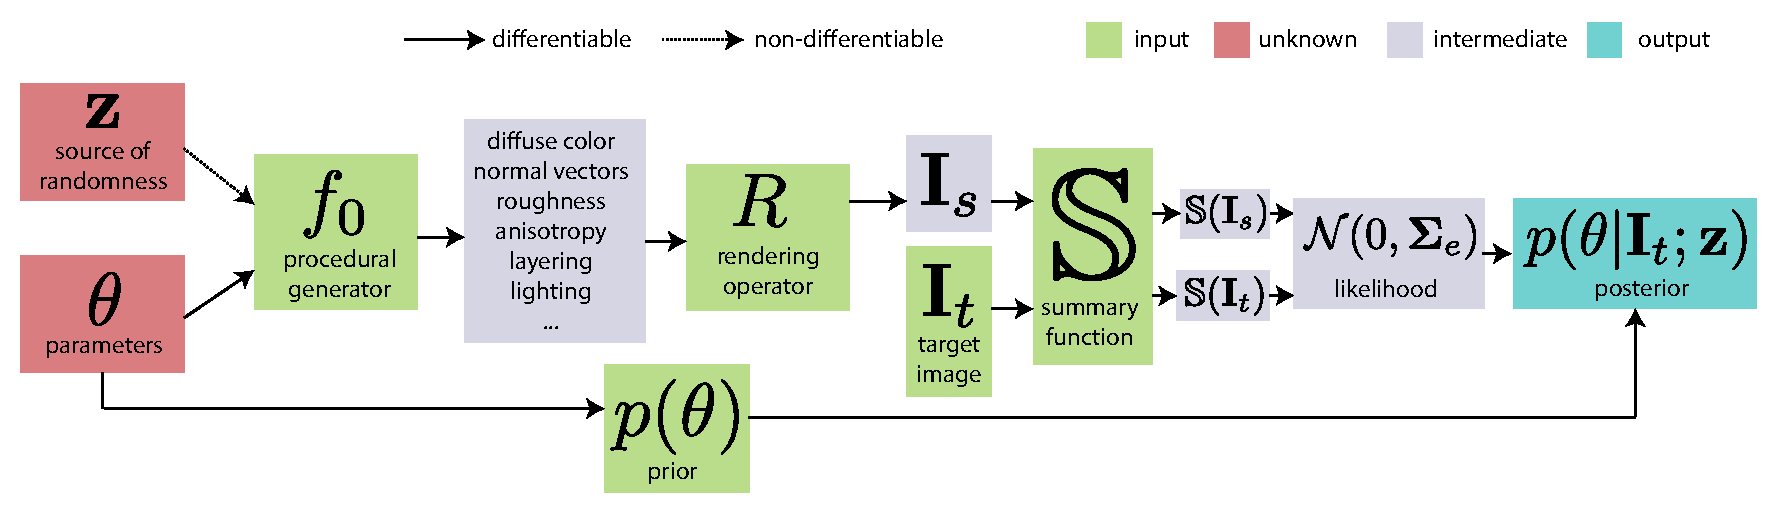
\includegraphics[width=\textwidth]{bayesian/fig1-2/posterior.pdf}
	\caption[Pipeline]{\label{fig:baesian:pipeline}
		Our posterior computation combines priors, a procedural material model, a rendering operator, a summary function, and a target image. This posterior distribution can then be sampled to provide plausible values of the parameter vector. The value of the posterior is computed up to a normalization term, which does not effect MCMC sampling. The entire posterior definition is differentiable in the material parameters (excluding optional discrete model parameters).}
\end{figure}

Our second contribution is to introduce a \emph{Bayesian inference} approach capable of drawing samples from the space of plausible material parameters.
This provides additional information beyond single point estimates of material parameters (for example, though not limited to, discovering similarity structures in the parameter space).
Further, due to an ability to combine multiple Markov-Chain Monte Carlo (MCMC) sampling techniques such as Metropolis-Hasting (MH), Hamiltonian Monte Carlo (HMC), and Metropolis-adjusted Langevin algorithm (MALA), our technique is capable of efficiently handling both discrete and continuous model parameters.
Posterior sampling is a well-studied area within statistics and has been used in computer vision and inverse rendering \cite{kulkarni2015picture}, but to our knowledge, it has not yet been applied to material appearance acquisition.

To demonstrate the effectiveness of our framework, we fit procedural models for a diverse set of materials from standard opaque dielectrics (e.g. plastics, leather, wall paint) to dielectrics with 3D structure (wood) to anisotropic brushed metals and layered metallic paints (see Figure~\ref{fig:bayesian:teaser}, \S\ref{sec:bayesian:results}, and the supplemental materials).

